% ----------------------------------------------------------------
%% Thesis.tex -- MAIN FILE (the one that you compile with LaTeX)
%% ---------------------------------------------------------------- 

% Set up the document
\documentclass[a4paper, 11pt, oneside]{Thesis}  % Use the "Thesis" style, based on the ECS Thesis style by Steve Gunn
%\graphicspath{Figures/}  % Location of the graphics files (set up for graphics to be in PDF format)
\usepackage{fancyhdr}
% Include any extra LaTeX packages required
\usepackage[square, numbers, comma, sort&compress]{natbib}  % Use the "Natbib" style for the references in the Bibliography
\usepackage{verbatim}  % Needed for the "comment" environment to make LaTeX comments
\usepackage{vector}  % Allows "\bvec{}" and "\buvec{}" for "blackboard" style bold vectors in maths
\usepackage{graphicx} 
\usepackage{pdfpages}
\usepackage{float}  % Required for the [H] option in figures
\usepackage{acronym} % Required for the acronym environment
\usepackage[autostyle,german=quotes]{csquotes} % Required for the \enquote command
\usepackage{amsmath}  % Required for the \text command in maths mode
\usepackage{subfigure}
\usepackage{subcaption} % Add this line to your preamble
\hypersetup{urlcolor=blue, colorlinks=true}  % Colours hyperlinks in blue, but this can be distracting if there are many links.
%
\pagestyle{fancy}
\fancyhf{}  % Alle Kopfzeilen löschen
%% ----------------------------------------------------------------
\renewcommand{\chaptername}{Kapitel}
\renewcommand{\tablename}{Tabelle}
\renewcommand{\bibname}{Literaturverzeichnis}
\renewcommand{\figurename}{Abbildung}
%% ----------------------------------------------------------------
\begin{document}
\begin{titlepage}

\newcommand{\HRule}{\rule{\linewidth}{0.5mm}} % Defines a new command for the horizontal lines, change thickness here

\center % Center everything on the page
 %----------------------------------------------------------------------------------------
%	LOGO SECTION
%----------------------------------------------------------------------------------------
\begin{minipage}{0.4\textwidth}
\begin{flushleft} \large

\includegraphics[width=5cm, height=1.2cm]{Pictures/UST.jpg}
\end{flushleft}
\end{minipage}

\begin{minipage}{0.4\textwidth}
\begin{flushright} \large

\includegraphics[width=5cm, height=1.2cm]{Pictures/ILH.jpg}
\end{flushright}
\end{minipage}\\[2cm]
 % Include a department/university logo - this will require the graphicx package
%----------------------------------------------------------------------------------------
%	HEADING SECTIONS
%----------------------------------------------------------------------------------------

\textsc{\LARGE \bfseries Fachpraktikum (Bachelor)}\\[0.2cm] % Name of your university/college
\textsc{\LARGE 6G Hardwarelabor - Design und Implementierung eines HF Transceivers}\\[0.2cm] 
%\textsc{\LARGE Design}\\[0.5cm] 
%\textsc{\Large ILH}\\[0.5cm] % Major heading such as course name
%\textsc{\large PuL-Analog Microwave Frontend Design}\\[0.5cm] % Minor heading such as course title

%----------------------------------------------------------------------------------------
%	TITLE SECTION
%----------------------------------------------------------------------------------------

\HRule \\[0.4cm]
{ \huge \bfseries Versuch 3: Design  und Simulation eines Coupled-Line Filters}\\[0.4cm] % Title of your document
\HRule \\[1.5cm]
 
%----------------------------------------------------------------------------------------
%	AUTHOR SECTION
%----------------------------------------------------------------------------------------
\textbf{Protokollführer}\\
{\large\ Lukas Müller}\\[0.2cm]
{\large\ Erik Zimmermann}\\[0.2cm]
{\large\ Farhad Valizada}\\[0.7cm]

\textbf{Betreuer}\\
{\large\ Simon Haussmann}\\[0.2cm]




%----------------------------------------------------------------------------------------
%	DATE SECTION
%----------------------------------------------------------------------------------------
\textbf{Eingereicht}\\
{\large \today} % Date, change the \today to a set date if you want to be precise

 
%----------------------------------------------------------------------------------------

\vfill % Fill the rest of the page with whitespace

\end{titlepage}


%\vfill\vfill\vfill\vfill\vfill\vfill\null
\clearpage  % Funny Quote page ended, start a new page
%% ----------------------------------------------------------------

\clearpage

\pagenumbering{arabic}
\pagestyle{fancy}
\fancyhf{}
\fancyfoot[C]{\thepage} % Seitenzahl unten zentriert
\renewcommand{\headrulewidth}{0pt}

% Ensure every chapter resets the pagestyle to fancy
\let\oldchapter\chapter
\renewcommand{\chapter}{\clearpage\pagestyle{fancy}\oldchapter}


% The Abstract Page


%% ----------------------------------------------------------------

\setstretch{1.3}  % Reset the line-spacing to 1.3 for body text (if it has changed)

% The Acknowledgements page, for thanking everyone
%\acknowledgements{
%\addtocontents{toc}{\vspace{1em}}  % Add a gap in the Contents, for aesthetics
%
%The acknowledgements and the people to thank go here, don't forget to include your project advisor\ldots
%
%}
%\clearpage  % End of the Acknowledgements1
%% ----------------------------------------------------------------

%\pagestyle{fancy}  %The page style headers have been "empty" all this time, now use the "fancy" headers as defined before to bring them back




\renewcommand{\contentsname}{Inhaltsverzeichnis}
\tableofcontents
\newpage

\chapter*{Abkürzungsverzeichnis}
\addcontentsline{toc}{chapter}{Abkürzungsverzeichnis}
\begin{acronym}[XXXXXX] % Adjust the width of the longest acronym
    \acro{ADS}{Advanced Design System}
    \acro{HF}{Hochfrequenz}
    \acro{6G}{Sixth Generation}
    \acro{SMA}{SubMiniature version A}
    \acro{PCB}{Printed Circuit Board}
\end{acronym}
\clearpage  % End of the Abkürzungsverzeichnis
%% ----------------------------------------------------------------

\chapter{Einleitung}
\section{Relevanz der Funkübertragung im Alltag}
Jeden Tag nutzen wir Funkübertragungen in verschiedenen Formen, sei es durch WLAN, Bluetooth oder Mobilfunk. Diese Technologien ermöglichen es uns, Daten über große Entfernungen zu übertragen, ohne physische Verbindungen herstellen zu müssen. Die Grundlagen der Modulation sind entscheidend für die Entwicklung und Verbesserung dieser Technologien.
Die \ac{6G} der Funkübertragung ist die neueste Generation der Funkkommunikation, die eine höhere Datenrate, geringere Latenz und verbesserte Zuverlässigkeit verspricht. Sie ist aktuell in der Entwicklung, 
jedoch besteht bei dem Frequenzbereich von \ac{6G}, beginnend mit Sub-6 GHz (unter 6 GHz) bis hin zu THz-Bereich (100 GHz - 1 THz), 
die Herausforderung, dass die Signale bei höheren Frequenzen stärker gedämpft werden und somit eine höhere Signalstärke erforderlich ist, um eine zuverlässige Kommunikation zu gewährleisten.
Deswegen ist es leichter, eine beispielhafte Funkübertragung bei kleineren Abständen zu dimensionieren, um das Wissen bei größeren Strecken anwenden zu können.
\section{Ziel des Versuchs}
Das Ziel des heutigen und des letzten Versuchs ist es, eine Bildübertragung über eine Funkverbindung zu realisieren und dabei die Grundlagen der Bildübertragung mithilfe von 6G zu verstehen.
Dies bietet einen guten Einblick in die digitale Kommunikation und die Modulation von Signalen, die für die Übertragung von Daten über Funkverbindungen unerlässlich ist.
\clearpage 

\chapter{Theoretische Grundlagen}
\section{Modulationsarten}

\section{Blockdiagramm einer Sendestrecke}
\subsection{DAC}
\subsection{LO}
\subsection{Mischer} 
\subsection{PA}
\subsection{Antennen}
\subsection{LNA}
\subsection{Demodulation}
\subsection{ADC}
\section{Mathematische Grundlagen: Fourier-Transformation}
\subsection{Betrag und zeitlicher Verlauf von Rechteckfunktion}
\subsection{Betrag und zeitlicher Verlauf von Sinusfunktion}
\subsection{Multiplikation der beiden Funktionen im Zeitbereich}
\section{Zusammenhang von Datenrate und Bandbreite}
blabla
\clearpage

\chapter{Verwendete Geräte und Messaufbau}

\section{Verwendete Geräte}
In diesem Versuch wurden folgende Geräte verwendet:
\begin{itemize}
    \item \textbf{Keysight Fieldfox Network Analyzer N9918A}: Zur Messung der S-Parameter des Filters.
    \item \textbf{Signal Generator}: Zur Erzeugung eines Testsignals, das durch den Filter geleitet wird.
    \item \textbf{Coupled-Line-Filter}: Das zu messende Filter, das in ADS entworfen und simuliert wurde. (siehe Schaltplan\_PCB\_V4)
\end{itemize}
\clearpage

\chapter{Praktische Umsetzung}
\begin{enumerate}
    \item Die PCB mit dem Coupled-Line-Filter wird mit dem Fieldfox an beiden Ausgängen angeschlossen, 
    woraufhin die S-Parameter dessen im Network-Analyzer-Modus vermessen werden. Folgender Leistungsspektrum kommt zustande:
    %     \begin{figure}[H]
    %         \centering
    %         \includegraphics[width=0.8\textwidth]{Pictures/Fieldfox_S-Parameter.png}
    %         \caption{S-Parameter des Coupled-Line-Filters}
    %         \label{fig:fieldfox_s_parameter}
    \item Als nächstes wird der Filter von dem Fieldfox abgekoppelt und
    \item Der Network Analyzer wurde so konfiguriert, dass er die S-Parameter des Filters misst.
\end{enumerate}
\section{Messung der S-Parameter im NA-Modus}
\section{Anschluss an den Transmitter und Messung im SA-Modus}
\section{Vergleich des gefilterten und ungefilterten Spektrums}


\chapter{Simulation mit ADS}
\section{Einrichtung des ADS-Workspaces}

    \subsection{Auswahl der Technologie und Erstellung des Substrat-Files}
    Bevor wir in ADS die Leitungen Simulieren können, muss das Substrat file definiert werden.
    Hier lässt sich die dicke der Kupferleitung sowie von dem Dielektrikum FR4 wählen.
        \begin{itemize}
            \item FR4    : 1mm
            \item Kupfer : 35\textmu m
        \end{itemize}
        \begin{figure}[H]
            \centering
            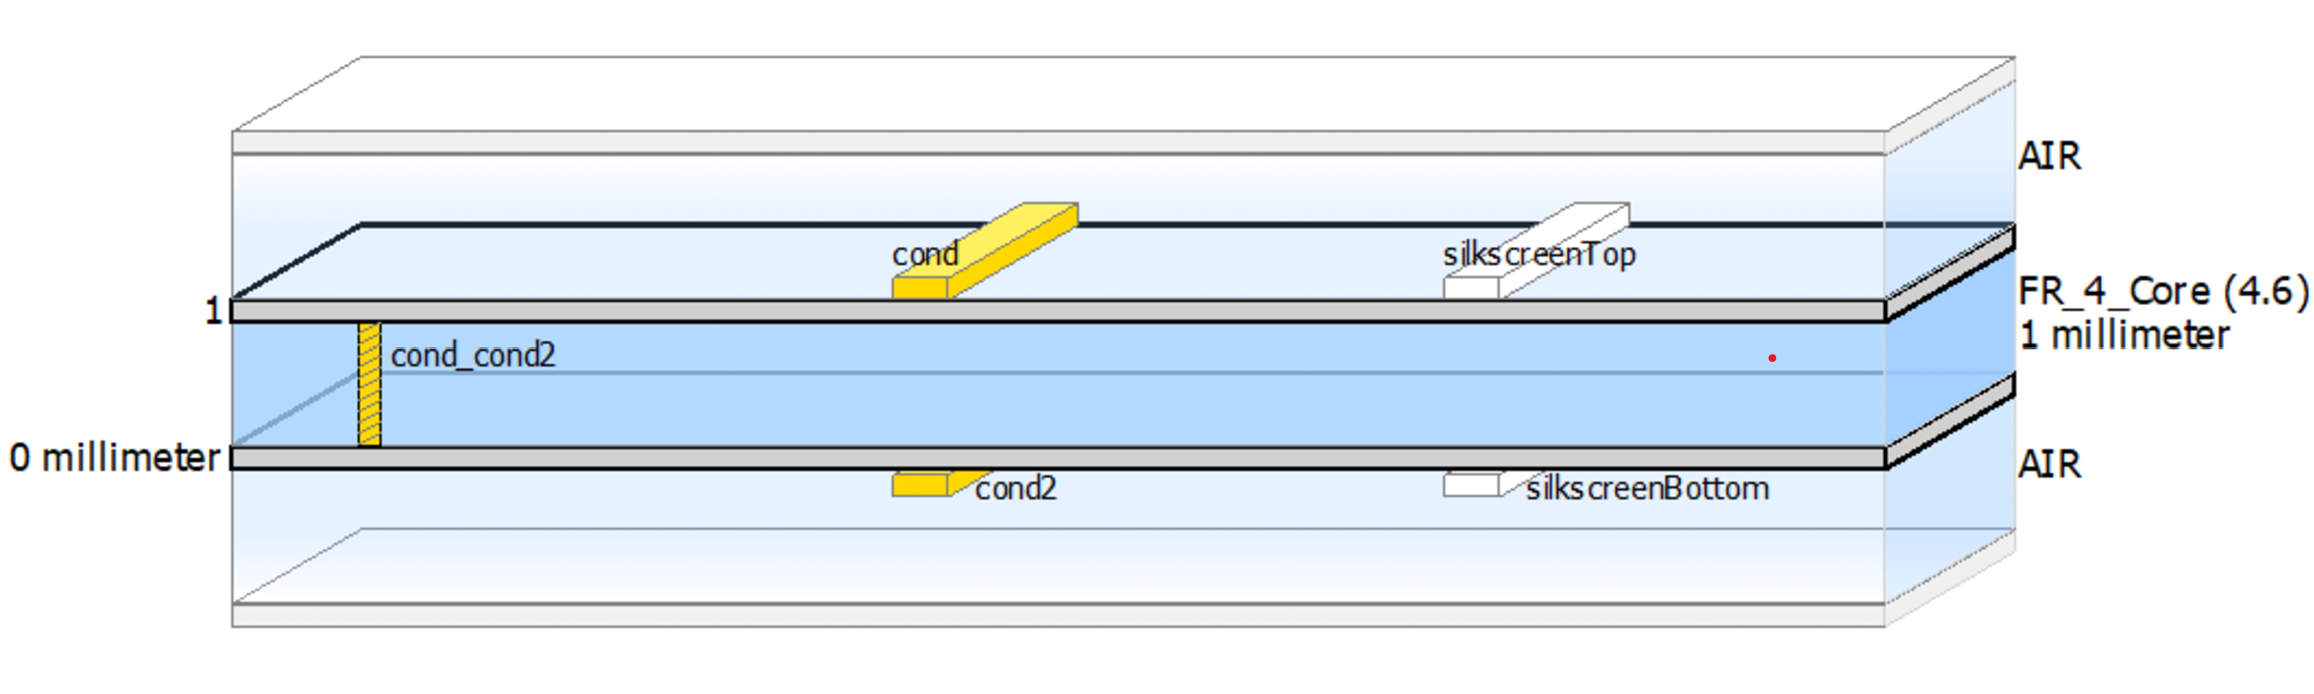
\includegraphics[width=0.9\textwidth]{Pictures/substratFile.png}
            \caption{Substratfile}
        \end{figure}

    \subsection{Nutzung des Controlled Impedance Line Designers}

\section{Leitungsdimensionierung}
    \subsection{\texorpdfstring{Berechnung der Leitungsbreite ($Z_0 = 50~\Omega$)}{Berechnung der Leitungsbreite (Z0 = 50 Ohm)}}
    Nun wird die Leitungsbreite einer Microstrip Leitung mit der Wellenimpedanz $Z_0 = 50~\Omega$ berechnet.
    Dazu verwenden wir die Formeln, die uns auf der Website von Microwaves101 Kapitel Microstrip zur
    Verfügung gestellt werden. Durch eine grobe Abmessung der Leitungsbreite sieht man das folgende Beziehung gilt: \\
    \[
    \frac{w}{h} \geq 1
    \]
    $w$ ist hier die Leitungsbreite und $h$ die Höhe des Dielektrikums. In unserem Fall ist $h = 1mm$ und $w$ wird variiert. Die 
    effektive Permitivität wird mit folgender Formel berechnet:
      \[
    \varepsilon_e = \frac{\varepsilon_r + 1}{2} + \frac{\varepsilon_r - 1}{2} \left( 1 + 12 \frac{h}{w} \right)^{-\frac{1}{2}}
    \]
   \\ $\varepsilon_e$ wird in die Formel zur Leitungsimpedanz eingesetzt. Bei dieser wird $w$
    variiert, bis die Wellenimpedanz $Z_0 = 50~\Omega$ erreicht wird.
    \\
    Die Formel zur Leistungsimpedanz $Z_o$ lautet:
    \[
    Z_0 = \frac{120 \pi}{\sqrt{\varepsilon_{\text{eff}}} \left( \frac{w}{h} + 1.393 + \frac{2}{3} \ln\left( \frac{w}{h} + 1.444 \right) \right)} \quad \text{(Ohm)}
    \]
    Die Berechnung der Leitungsbreite wird hierbei numerisch durchgeführt, da eine analytische Berechnung zu
    komplex werden würde. Die Ergebnisse der Approximation werden in Tablle 4.1 dargestellt. \\
    
    \begin{table}[H]
        \centering
        \begin{tabular}{|l|l|}
            \hline
            \textbf{Leitungsbreite $w$ (mm)} & \textbf{Wellenimpedanz $Z_0$ ($\Omega$)} \\
            \hline
            1.7 & 52.749 \\
            1.8 & 51.027 \\
            1.9 & 49.419 \\
            2.0 & 47.915 \\
           
            \hline
        \end{tabular}
        \caption{Berechnete Wellenimpedanz für verschiedene Leitungsbreiten}
    \end{table}
    Anhand der berechneten Werte liegt die Leitungsbreite mit $w = 1.8~mm$ am nähesten an der Wellenimpedanz.
    Eine nähere Berechnung ist mit unserem TR nicht möglich. 

       

    \subsection{Verifizierung der Berechneten Leitungsbreite}
    Nun wird die Leitungsbreite mithilfe des Controlled Impedance Line Designers Simuliert.
    Ziel ist es die $Z_0 = 50~\Omega$ zu erreichen durch sweepen der Leitungsbreite
    \begin{figure}[H]
        \centering
        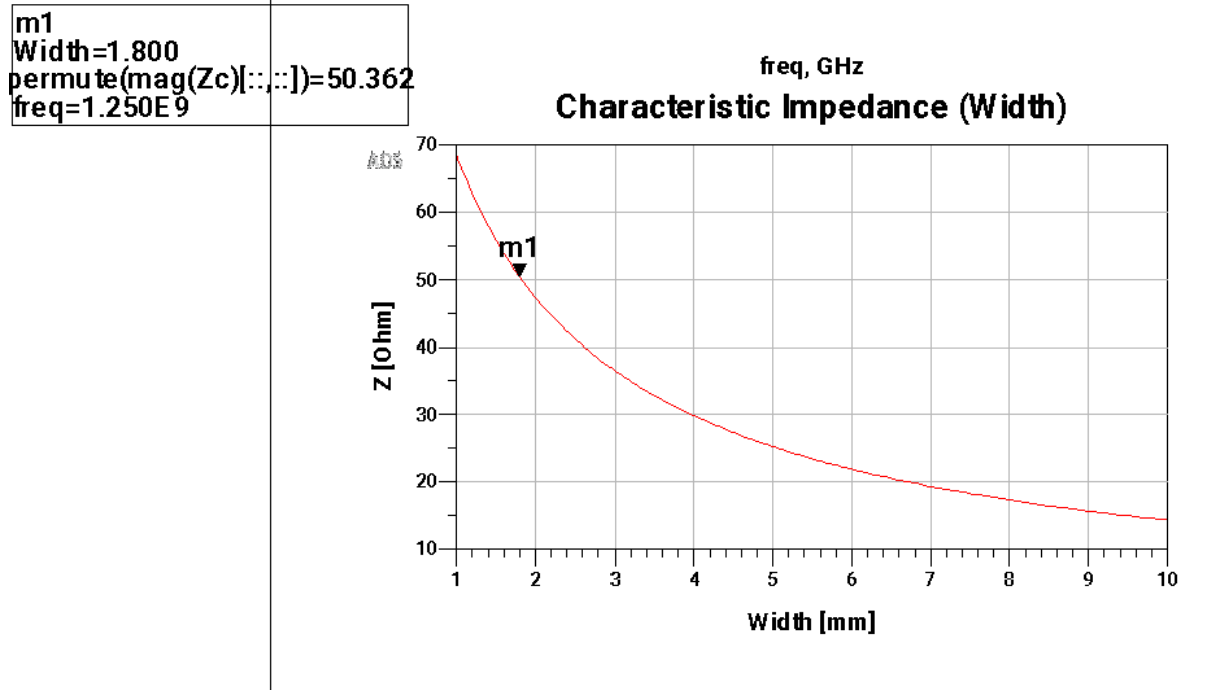
\includegraphics[width=0.8\textwidth]{Pictures/LeitungsbreitenSweep.png}
        \caption{Wellenimpedanz in abhängigkeit von der Leitungsbreite}
    \end{figure}
    Wie schon numerisch bestimmt kommen wir mitn der Leiterbreite $w=1.8mm$ der Wellenimpdanz $Z_0 = 50~\Omega$
    am nähesten. Würde man noch genauer sweepen, wird man festellen dass die Optimale Leiterbreite irgendwo zwischen
    $1.8mm$ und $1.9mm$ liegt.

    \subsection{Charakteristische Länge der Koppelleitungen}
    \subsection{Bestimmung der Filterordnung}

\section{Aufbau des Coupled-Line-Filters im Schematic}

\section{Simulation und Optimierung}
    \subsection{Vergleich mit Messdaten}

\section{Knick zur Optimierung des Aspektverhältnisses}

\section{Anpassung im Schematic und Re-Simulation}

\section{Auswirkungen auf die S-Parameter}



\chapter{Fazit}

Im Verlauf dieses Versuches konnten wir die grundlegende Funktionsweise eines Coupled Line Filters praktisch nachvollziehen und ebenfalls unser theoretisches Wissen erweitern. Es ist sehr interessant zu sehen, wie sich die anfangs unscheinbaren Platine zu einem komplexen Konstrukt entwickelt deren einzelnen Komponenten und deren Zusammenspiel wir nach und nach immer besser verstehen. Ebenfalls ist die Arbeit mit der Simmulationssofware ADS äußerst erkenntnisreich und hilft uns die Fehler in dem praktischen Teil des Versuches zu identifizieren und zu sehen, wie es unter optimalen Bedingungen aussehen müsste. Es gibt noch vieles zu lernen im Verlauf dieses Praktikums und wir sind gespannt auf das was noch kommt. 
\clearpage  

\renewcommand{\bibname}{Literaturverzeichnis}
\addcontentsline{toc}{chapter}{Literaturverzeichnis}
\input{Chapter/literaturverzeichnis}






\end{document}  % The End
%% ----------------------------------------------------------------